\documentclass[11pt]{beamer}
\usepackage[utf8]{inputenc}
\usepackage[T1]{fontenc}
\usepackage{datetime}

\usepackage{graphicx}
\usepackage{algorithm}
\usepackage{algpseudocode}

% Remove these 2 lines
\usepackage[english]{babel}
\usepackage{blindtext}

% Defining a color
\usepackage{xcolor}
\definecolor{uwo-purple}{HTML}{4F2683}
\definecolor{uwo-gray}{HTML}{807F83}

\usetheme{CambridgeUS}

% Customizing the template
\setbeamercolor{frametitle}{fg=uwo-purple}
\setbeamercolor{title}{fg=uwo-purple}
\setbeamercolor{palette primary}{fg=black, bg=uwo-purple!30!white}
\setbeamercolor{palette secondary}{fg=black, bg=uwo-purple!20!white}
\setbeamercolor{palette tertiary}{bg=uwo-purple}

\newcommand{\bigo}{\mathcal{O}}
\newcommand{\ZZ}{\mathbb{Z}}
\newcommand{\NN}{\mathbb{N}}
\newcommand{\LCM}{\operatorname{LCM}}
\newcommand{\wt}{\widetilde}

\begin{document}
  \author[Kumar]{Kumar Sannidhya Shukla \\ \tiny\hyperlink{mailto:kshukla5@uwo.ca}{kshukla5@uwo.ca}}
  \newdate{date}{28}{06}{2023}
  \date{\displaydate{date}}
  \title[AKS]{Deterministic Polynomial-Time Primality Testing}
  \subtitle{The AKS Primality Testing Algorithm}
  \logo{
\includegraphics[width=1cm]{resources/Stacked_CMYK}}
  \institute[Math]{Department of Mathematics}
  \subject{Math 9171L - Mathematical Computation}
  %\setbeamercovered{transparent}
  %\setbeamertemplate{navigation symbols}{}

\begin{frame}
  \maketitle
  \centering
  Math 9171L - Mathematical Computation
\end{frame}

\section*{Overview}
\begin{frame}
\frametitle{Outline}
\tableofcontents
\end{frame}

\section{Pre AKS: Eratosthenes, Fermat }

\begin{frame}
\frametitle{Sieve of Eratosthenes}
An algorithm to generate all primes up to $n$.
\centering
\begin{itemize}
  \item Start with a list of numbers $\{2, \dots, n\}$
\end{itemize}
    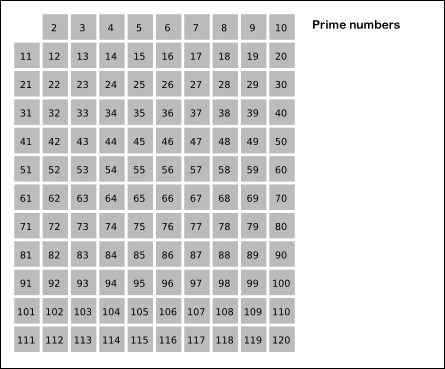
\includegraphics[scale=0.45]{resources/sieve-0.jpg}
\end{frame}

\begin{frame}
\frametitle{Sieve of Eratosthenes}
\centering
\begin{itemize}
  \item  Add $2$ to  the list of primes.
\end{itemize}
    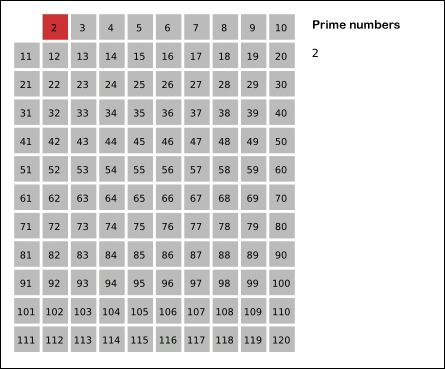
\includegraphics[scale=0.45]{resources/sieve-1.jpg}
\end{frame}

\begin{frame}
\frametitle{Sieve of Eratosthenes}
\centering
\begin{itemize}
  \item Drop all multiples of $2$.
\end{itemize}
    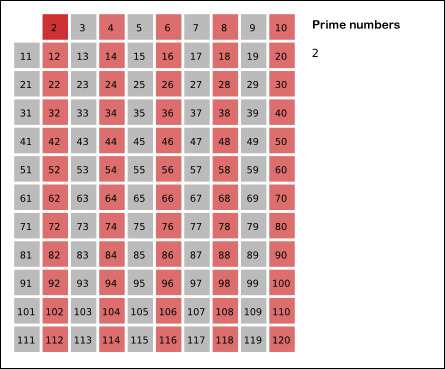
\includegraphics[scale=0.45]{resources/sieve-60.jpg}
\end{frame}

\begin{frame}
\frametitle{Sieve of Eratosthenes}
\centering
\begin{itemize}
  \item  Add $3$ to  the list of primes.
\end{itemize}
    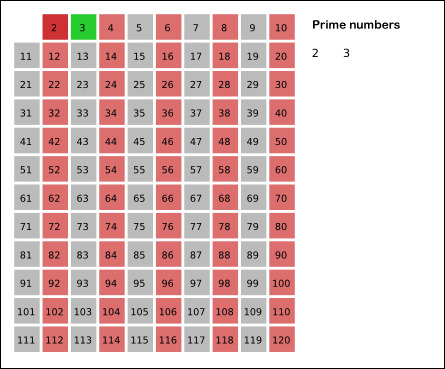
\includegraphics[scale=0.45]{resources/sieve-61.jpg}
\end{frame}

\begin{frame}
\frametitle{Sieve of Eratosthenes}
\centering
\begin{itemize}
  \item Drop all multiples of $3$.
\end{itemize}
    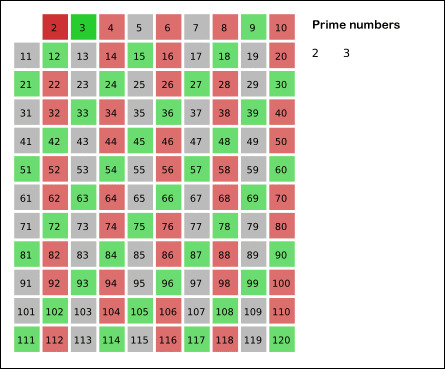
\includegraphics[scale=0.45]{resources/sieve-99.jpg}
\end{frame}

\begin{frame}
  \centering
\frametitle{Sieve of Eratosthenes}
\begin{itemize}
  \item  Add $5$ to  the list of primes.
\end{itemize}
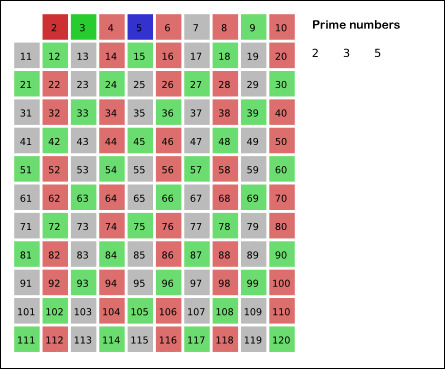
\includegraphics[scale=0.45]{resources/sieve-100.jpg}
\end{frame}

\begin{frame}
\frametitle{Sieve of Eratosthenes}
\centering
\begin{itemize}
  \item Drop all multiples of $5$.
\end{itemize}
    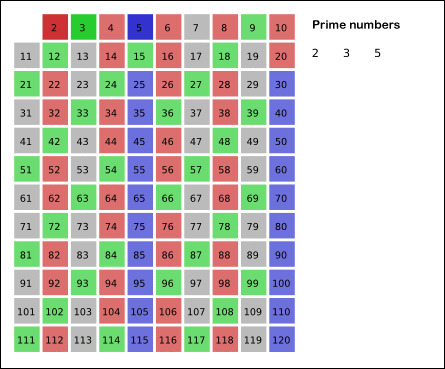
\includegraphics[scale=0.45]{resources/sieve-120.jpg}
\end{frame}

\begin{frame}
\frametitle{Sieve of Eratosthenes}
\centering
\begin{itemize}
  \item ...
\end{itemize}
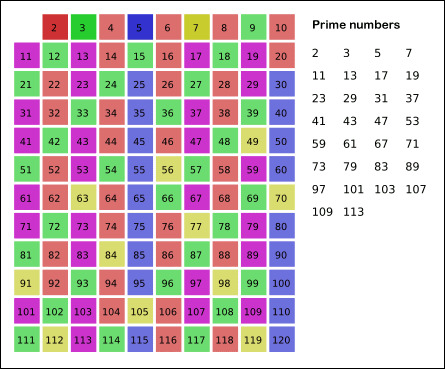
\includegraphics[scale=0.45]{resources/sieve-158.jpg}
\end{frame}

\begin{frame}
\frametitle{Sieve of Eratosthenes}
An algorithm to generate all primes up to $n$.
\begin{algorithm}[H]
\caption{Seive of Eratosthenes}\label{alg:cap}
\begin{algorithmic}[1]
  \State \textbf{Input.} n
  \State $L = [1, n]$
  \State $i = 1$
  \While {$i < len(L)$}
    \For {$ j = 2 \to \lfloor n/i \rfloor$}
      \State Delete L[i]*j from L
    \EndFor
  \EndWhile
  \State \Return L
\end{algorithmic}
\end{algorithm}

Runtime: $\bigo(2^{\log n})$

\end{frame}

\begin{frame}
\frametitle{Fermat's Primality Test}
\begin{theorem}[Fermat's little theorem]
  Let $p$ be a prime then $a^{p} \equiv a \mod p$
\end{theorem}
This can theorem can be used to devise a primality test as follows:
\begin{itemize}
  \item Given a number $n$
  \item Pick a random $a, 1 < a < n$
  \item Test whether $a^n \equiv a \mod n$
  \item If false, return \texttt{Composite}
  \item Otherwise, return \texttt{Prime}
\end{itemize}
\end{frame}

\begin{frame}
\frametitle{Fermat's Primality Test}
\begin{theorem}[Fermat's little theorem]
  Let $p$ be a prime then $a^{p} \equiv a \mod p$
\end{theorem}
This can theorem can be used to devise a primality test as follows:
\begin{enumerate}
  \item Given a number $n$
  \item Pick a random $a, 1 < a < n$
  \item Test whether $a^n \equiv a \mod n$
  \item Run the above steps multiple times
  \item If the congruence in step 3 is false even once, return \texttt{Composite}
  \item Otherwise, return \texttt{Prime}
\end{enumerate}
\end{frame}

\begin{frame}
\frametitle{Fermat's Primality Test}
\begin{algorithm}[H]
\caption{Fermat's Primality Test}\label{alg:fermat}
\begin{algorithmic}[1]
  \State \textbf{Input.} n
  \For{$i = 1 \to 10$}
  \State Generate random $a$, $1 < a < n$.
  \If {$a^n \not\equiv a \mod n$}
    \State \Return \texttt{Composite}
  \EndIf
  \EndFor
  \State \Return \texttt{Prime}
\end{algorithmic}
\end{algorithm}
\end{frame}

\begin{frame}
\frametitle{Fermat's Primality Test}
\begin{definition}[Carmichael numbers]
  A Carmichael number is a composite number $n$, such that
  $a^n \equiv a \mod n$ for all $1 < a < n$.
\end{definition}
\textbf{Example.} 561, 1729, 2465, etc.\\
\pause
Carmichael numbers will fool Fermat's test 100\% of the times!\\
\pause
There are infinitely many Carmichael numbers!!
\end{frame}

\section{Generalized Fermat's Theorem}
\begin{frame}
  \frametitle{Generalized Fermat's Theorem}
  \begin{theorem}
    Let $n > 1$ and $a \in \ZZ_n^*$. Then $n$ is a prime if and only if
  \[
    (x+a)^n = x^n + a
  \]
  in $\ZZ_n[x]$.
  \pause
  \begin{proof}
  If $n$ is a prime, then $n \big| {n \choose k}$ for all $k$.\\
  \pause
  If $n$ is a composite, suppose $n = p^k.m$, $p \not| m$. Then,
  $p^k \not\big| {n \choose  p}a^{n-p}$.
  \end{proof}
  \end{theorem}
\end{frame}

\begin{frame}
  \frametitle{Examples}
  \begin{example}
    The number $5$ is a prime. So,
    \[
      (x+1)^5 = x^5 + 5x^4 + 10x^3 + 10x^2 + 5x + 1 = x^5 + 1 \text{ in }
      \ZZ_5[x].
    \]
  \end{example}
  \pause
  \begin{example}
    The number $4$ is not a prime. So,
    \begin{align*}
      (x+1)^4 & = x^4 + 4x^3 + 6x^2 + 4x + 1 \\
              & = x^4 + 2x^2 + 1 \\
              & \not= x^4 + 1 \text{ in } \ZZ_4[x].
    \end{align*}
  \end{example}
\end{frame}

\section{The AKS Primality Test}
\begin{frame}
  \frametitle{Reduction mod $x^r - 1$}
  \begin{itemize}
    \item If we naively try to turn the generalized Fermat's little theorem
      into a primality test, then we get exponential runtime.
    \item The idea is to reduce the number of coefficients by modding
      out by $x^r - 1$.
    \item The ring to consider: $\ZZ_n[x]/(x^r - 1)$.
    \item $ x^n + a = x^{n \mod r} + a $
  \end{itemize}
\end{frame}

\begin{frame}
  \frametitle{How to choose $r$?}
  \begin{itemize}
    \item r should be small so that enough coefficients of $(x + a)^n$ 
      get killed but not so small that composite numbers don't satisfy
      the congruence.
  \end{itemize}
  \begin{theorem}
    There exist an $r$, $3 \le r \le \lceil \log^5 n\rceil$, such that
    $o_r(n) > \lfloor \log^2 n\rfloor$.
  \end{theorem}
  \begin{proof}
    Suppose for all $r \le R$, we have $o_r(n) \le \lfloor \log^2 n \rfloor$.
    Then, $r | (n-1)(n^2 - 1)\dots(n^{\lfloor \log^2 n \rfloor} - 1) = P$.\\
    So, $\LCM\{r : 1 \le r \le R\} | P$.
    By LCM bound, $2^R \le P$.
    Thus, $R < \log^5 n$.
  \end{proof}
\end{frame}

\begin{frame}
  \frametitle{The AKS Algorithm}
\begin{algorithm}[H]
\caption{AKS Primality Test}\label{alg:aks}
\begin{algorithmic}[1]
  \State \textbf{Input.} n
  \If{$n = a^b$, $a, b > 1$}
  \State \Return \texttt{Composite}
  \EndIf
  \State Find $r$, such that $o_r(n) > \log^2 n$
  \If {$\exists a\in [r], 1 < (a, n) < n$}
  \State \Return \texttt{Composite}
  \EndIf
  \For{$a = 1 \to \lceil 2\sqrt{r}\log{n} \rceil$}
  \If{$(x + a)^n \ne x^n + a \text{ in } \ZZ_n[x]/(x^r - 1)$}
  \State \Return \texttt{Composite}
  \EndIf
  \EndFor
  \State \Return \texttt{Prime}
\end{algorithmic}
\end{algorithm}
\end{frame}

\section{Proof of Correctness}
\begin{frame}
  \frametitle{Proof of Correctness}
\begin{theorem}
  The AKS test returns \texttt{Prime} if and only if then input $n$ is prime.
\end{theorem}
\begin{proof}
  $(\impliedby)$ Obvious.\\
  $(\implies)$ Suppose conversely that the algorithm
  returns $\texttt{Prime}$. In particular this means, that all congruences
  in line 10 hold true. Suppose the $n$ has a prime factor $p$. We will
  show that $n = p$.

  Define a group,
  \[
    I := \langle p, n \mod r\rangle
  \]
  \[
    t := |I| \ge o_r(n) > \log^2 n
  \]
\end{proof}
\end{frame}

\begin{frame}
  \frametitle{Proof of Correctness}
  \begin{proof}(Continued.)
    Let $h(x)$ be an irreducible factor of $(x^r-1)/(x-1)$. Then, $\ZZ_p[x]/(h(x))$
    is a field.
    Define another group,
  \[
    J := \langle x+1, x+2, \dots, x+ r \mod (p, h)\rangle
  \]
  \[
    |J| > n^{2\sqrt{t}}
  \]
  $J$ is a cyclic group, let $f$ be a generator of $J$.
\end{proof}
\end{frame}

\begin{frame}
  \frametitle{Proof of Correctness}
  \begin{proof}(Continued.)
    There exist $(i, j) \ne (i', j')$, $0 \le i, j, i', j' \le \sqrt{t}$
    such that $n^{i}p^{j} = n^{i'}p^{j'}$. Then,
    \[
      f(x^{n^{i}p^j}) = f(x^{n^{i'}p^{j'}}) \text{ in } \ZZ_p[x]/(h(x))
    \]\[
      f(x)^{n^{i}p^j} = f(x)^{n^{i'}p^{j'}} \text{ in } \ZZ_p[x]/(h(x))
    \]\[
      {n^{i}p^j} = {n^{i'}p^{j'}} \mod |J|
    \]
    So $n$ is a prime power, but we already rejected all higher powers,
    so $n$ must be a prime.
  \end{proof}
\end{frame}

\section{Time Complexity}
\begin{frame}
  \frametitle{Arithmetic in $\ZZ_p$ and $\ZZ_p[x]/(q(x))$}
  \begin{itemize}
    \item \textbf{Notation.} $\wt{\bigo}(f(n)) = \bigo(f(n)\cdot\texttt{poly}(\log f(n)))$
    \item Multiplication in $\ZZ_p$: $\bigo(\log p \cdot (\log \log p)^2) = \wt\bigo(\log p)$
    \item Multiplication in $\ZZ_p[x]/(q(x))$: $\wt\bigo(r\log r\log p)$
      where $r = \deg q(x)$.
      
  \end{itemize}
\end{frame}

\begin{frame}
  \frametitle{Time Complexity}
  \begin{itemize}
    \item Perfect power test: $\wt\bigo(\log^3 n)$
    \item Finding appropriate value of $r$: $\wt\bigo(R\log^2 n) = \wt{\bigo}
      (\log^7 n)$.
    \item GCD step: $\wt\bigo(r \log n) = \wt\bigo(\log^6 n)$
    \item Generalized FLT step: $(\sqrt{r}\log n)\wt\bigo(r \log^2 n) = \wt\bigo(\log^{21/2} n)$
    \item Total complexity: $\wt\bigo(\log^{21/2} n)$
  \end{itemize}
\end{frame}

\section{Epilogue}

\begin{frame}
  \frametitle{Epilogue}
  \begin{itemize}
    \item Recall the language \texttt{PRIMES} of all prime
      numbers. 
      \[ \texttt{PRIMES} = \{p \in \NN : p \text{ is a prime}\}\]
    \item Then the existence of a deterministic polynomial
      time algorithm proves that
      \begin{theorem}[Agrawal-Kayal-Saxena, 2002]
        \texttt{PRIMES} is in P.
      \end{theorem}
  \end{itemize}
\end{frame}

\section{Source Code}

\begin{frame}
  Source code available on \url{https://github.com/feynhat/math9171}.
\end{frame}

\section{References}
\begin{frame}
\frametitle{References}
\begin{thebibliography}{10}

  \beamertemplatebookbibitems
  % Start with overview books.

  \bibitem{mnz}
    Ivan Niven, Herbert Zuckerman, Hugh Montgomery
    \newblock {\em An Introduction to the Theory of Numbers}.
    \newblock John Wiley \& Sons, 1991.

  \beamertemplatearticlebibitems
  % Followed by interesting articles. Keep the list short.

  \bibitem{aks}
    Manindra Agrawal, Neeraj Kayal, Nitin Saxena
    \newblock PRIMES is in P.
    \newblock {\em  Annals of Mathematics}, 2004.
  \end{thebibliography}
\end{frame}

\end{document}
